\documentclass[11pt,a4paper]{article}

% ── Packages ──────────────────────────────────────────────────────
\usepackage[utf8]{inputenc}
\usepackage[T1]{fontenc}
\usepackage{times}
\usepackage[margin=1in]{geometry}
\usepackage{graphicx}
\usepackage{booktabs}
\usepackage{amsmath,amssymb}
\usepackage{hyperref}
\usepackage{cleveref}
\usepackage{enumitem}
\usepackage{xcolor}
\usepackage{multirow}
\usepackage{caption}
\usepackage{subcaption}
\usepackage{natbib}
\bibliographystyle{plainnat}

\hypersetup{
    colorlinks=true,
    linkcolor=blue!60!black,
    citecolor=blue!60!black,
    urlcolor=blue!60!black,
}

\title{Zero-Shot Confidence Estimation for Small LLMs:\\When Supervised Baselines Aren't Worth Training}

\author{
    Anonymous Author(s)\\
    \textit{Anonymous Affiliation}\\
    \texttt{anonymous@example.com}
}

\date{}

\begin{document}
\maketitle

% ══════════════════════════════════════════════════════════════════
\begin{abstract}
Local-to-cloud LLM routing decides whether a cheap local model can answer a query or whether to escalate to an expensive cloud model. The dominant approach trains a supervised classifier on labeled routing examples. We ask whether that training is necessary.

We compare six zero-shot confidence signals against RouteLLM-style supervised baselines across three local model families (Qwen-2.5-7B, Llama-3.1-8B, Mistral-7B-Instruct) and two datasets (MMLU-Pro, TriviaQA; ${\sim}$3{,}000 evaluation queries per model). We find that (1)~average token log-probability, a zero-shot signal requiring no training data, matches or exceeds supervised baselines in-distribution (AUROC 0.650--0.714 vs.\ 0.644--0.676) and substantially outperforms them out-of-distribution (0.717--0.833 vs.\ 0.512--0.564); (2)~supervised routing transfers across model families but collapses on a new dataset; (3)~naive multi-signal fusion hurts rather than helps; and (4)~signal quality correlates with RLHF calibration training across model families. We provide a cold-start deployment guide and release all code, data, and experiment logs.
\end{abstract}

% ══════════════════════════════════════════════════════════════════
\section{Introduction}
\label{sec:intro}

Running a small local model (7--8B parameters) for most queries and escalating to a cloud model only when the local model is likely to fail is an increasingly common architecture for cost-sensitive LLM deployments. The routing decision---local or cloud?---determines both cost and quality. A growing body of work addresses this problem, but the field has converged on supervised approaches without adequately testing whether the supervision is necessary.

\subsection{Supervised Routing}

RouteLLM \citep{ong2024routellm} established the dominant paradigm: train a classifier on labeled (query, model-was-sufficient) pairs. Subsequent work extends this to contextual bandits under budget constraints \citep{chen2025adaptive}, bandit feedback with regret guarantees \citep{soare2025bandit}, dueling feedback \citep{li2025dueling}, and non-stationary settings where pricing and quality shift over time \citep{tabernermiller2026paretobandit}. \citet{gomes2025routing} survey routing strategies more broadly.

All of these approaches require training data---labeled examples, preference pairs, or online feedback. For a new deployment, this means generating answers from both local and cloud models on a representative corpus, labeling correctness, and fitting a routing model. In our experiments, this costs approximately \$25 and 2~hours per local model.

\subsection{Zero-Shot Confidence Signals}

An alternative extracts confidence signals directly from the local model's inference, with no training data.

\textbf{Token-level calibration.} \citet{kadavath2022language} showed that RLHF'd models produce calibrated token probabilities that correlate with correctness. \citet{guo2017calibration} established calibration theory for deep networks. \citet{huang2024logprob} demonstrated that log-probabilities remain reliable plausibility estimates in instruction-tuned models.

\textbf{Self-assessment.} \citet{kadavath2022language} tested P(True) prompting for self-evaluation. \citet{ren2023selfeval} reformulated generation into token-level self-evaluation, improving selective generation on TruthfulQA. \citet{chen2024trust} found self-reported confidence achieves better calibration than self-consistency at $5\times$ lower cost.

\textbf{Multi-signal uncertainty.} UQLM \citep{lin2025uqlm} and MUSE \citep{geng2025muse} combine multiple uncertainty signals into unified frameworks. \citet{mukkunnoth2025confidence} combine semantic alignment, internal convergence, and learned confidence for pre-generation hallucination routing. \citet{wang2022selfconsistency} introduced self-consistency---sampling multiple reasoning paths and measuring agreement---as a confidence proxy.

\subsection{Uncertainty-Based Routing}

The closest work to ours is \citet{chuang2025confident}, who benchmark uncertainty-based SLM-to-LLM routing across 1{,}500+ settings. They find that uncertainty distributions depend more on the SLM and quantification method than on downstream data, and propose a calibration data construction pipeline for generalization. \citet{zhang2025uncertainty} propose a confidence-driven router for edge-cloud deployment, evaluating on MT-Bench, GSM8K, and MMLU.

\subsection{The Gap We Address}

Despite this active literature, a specific comparison is missing. Existing routing papers assume supervision is available and do not benchmark against zero-shot alternatives. Existing confidence papers study signal quality in isolation without comparing to supervised routing baselines. \citet{chuang2025confident} benchmark uncertainty methods against each other, not against supervised routers. \citet{lugoloobi2026encode} demonstrate that linear probes on pre-generation activations can predict success and guide routing, but require access to model internals and per-model probe training; they do not compare against supervised baselines or test cross-dataset transfer. No published work evaluates zero-shot confidence signals against supervised routing baselines across multiple model families \emph{and} multiple datasets.

We fill this gap and find that the supervised approach is not worth the investment for most deployments.

\subsection{Contributions}

\begin{enumerate}[leftmargin=*,itemsep=2pt]
\item A cross-model, cross-dataset comparison of six zero-shot confidence signals against supervised baselines (3 models $\times$ 2 datasets $\times$ ${\sim}$1{,}000 queries each), with bootstrap CIs and paired significance tests.
\item The finding that supervised routing is dataset-specific while zero-shot log-probability transfers across both models and datasets (\S\ref{sec:cross-dataset}).
\item A learning curve showing supervised routing converges at ${\sim}$250 examples but never exceeds the zero-shot baseline (\S\ref{sec:learning-curve}).
\item Evidence that signal quality correlates with RLHF calibration training, with logprob and self-assessment complementary across the model-family axis (\S\ref{sec:analysis-logprob}).
\item A cold-start deployment guide (\S\ref{sec:deployment}) and a retrieval-conditional self-assessment design principle (\S\ref{sec:retrieval-gsa}).
\end{enumerate}

All experiments are reproducible on a single laptop with Ollama and AWS Bedrock. Total cloud cost: \$123.

% ══════════════════════════════════════════════════════════════════
\section{Signals and Baselines}
\label{sec:signals}

\subsection{Zero-Shot Confidence Signals}

We evaluate six signals computed at inference time without training data.

\textbf{Log-probability (logprob).} Average per-token log-probability of the local model's generated answer, mapped to $[0,1]$ via $\sigma(\bar{\ell} \cdot 2 + 3)$ where $\bar{\ell}$ is the mean token log-prob. Higher values indicate greater token-level confidence \citep{kadavath2022language}.

\textbf{Self-assessment (GSA).} A single-token YES/NO probe: the model is asked ``Are you confident you can answer this question correctly?'' and the YES-token probability is extracted from the first position's logprobs. We test a bare variant and a retrieval-conditional variant~(v3) that injects strong retrieved hits when available but falls back to a byte-identical bare prompt otherwise, so the model cannot distinguish ``retrieval found nothing'' from ``retrieval was never attempted.''

\textbf{Self-consistency (SC).} Jaccard token overlap between two independent generations at temperature 0.0 and 0.7 \citep{wang2022selfconsistency}.

\textbf{Knowledge similarity (KS).} Maximum cosine similarity between the query embedding and top-5 retrieved KB entries via FAISS inner-product on L2-normalized bge-large-en-v1.5 embeddings (1024-dim).

\textbf{Query classification (QC).} Keyword heuristic: factual $\to$ 0.7, real-time $\to$ 0.2, creative $\to$ 0.4, default $\to$ 0.5.

\textbf{Energy scorer (ES).} Logistic regression on query embeddings trained on the agent's pass/fail history. Disabled in all experiments (requires 50+ labeled examples).

\subsection{Supervised Baselines}

Following RouteLLM \citep{ong2024routellm}, we train two logistic regression classifiers (LogisticRegressionCV, 5-fold) on a disjoint 1{,}000-query training corpus per model:
\begin{itemize}[leftmargin=*,itemsep=1pt]
\item \textbf{RouteLLM-nm}: query embedding $\to$ $P(\text{local sufficient})$
\item \textbf{RouteLLM-pks}: $[\text{query embedding} \| \text{knowledge similarity}] \to P(\text{local sufficient})$
\end{itemize}

% ══════════════════════════════════════════════════════════════════
\section{Experimental Setup}
\label{sec:setup}

\subsection{Models}

\begin{table}[h]
\centering
\caption{Local models evaluated.}
\label{tab:models}
\begin{tabular}{lrl}
\toprule
Model & Params & RLHF emphasis \\
\midrule
Qwen-2.5-7B & 7.6B & Calibration-aware \\
Llama-3.1-8B-Instruct & 8.0B & Helpfulness / harmlessness \\
Mistral-7B-Instruct & 7.2B & Mixed \\
\bottomrule
\end{tabular}
\end{table}

Cloud model: Claude Sonnet~4.5 (AWS Bedrock). Judge: Claude Opus~4.5.

\subsection{Datasets}

\textbf{MMLU-Pro} (primary): 10-option MCQ, 14 categories. KB: 995 seeded entries. Eval: 931--999 queries per model.

\textbf{TriviaQA} (secondary): open-ended short-answer. KB: 200 seeded entries. Eval: 500 queries per model.

\subsection{Labeling}

MMLU-Pro uses regex letter extraction with LLM-judge fallback. TriviaQA uses standard substring matching.

\begin{table}[h]
\centering
\caption{Judge fallback rates on MMLU-Pro.}
\label{tab:judge}
\begin{tabular}{lrr}
\toprule
Model & Judge calls / total & Rate \\
\midrule
Qwen-2.5-7B & 688 / 931 & 74\% \\
Llama-3.1-8B & 755 / 997 & 76\% \\
Mistral-7B & 972 / 999 & 97\% \\
\bottomrule
\end{tabular}
\end{table}

Mistral's 97\% judge rate reflects poorly formatted responses; its AUROC is more sensitive to judge noise. Label noise bound: 13\% inter-judge disagreement (Opus vs.\ Sonnet audit on 100 rows). Differential comparisons are robust to symmetric noise.

\subsection{Evaluation Protocol}

AUROC with 1{,}000-sample bootstrap CIs (fixed seed). Paired deltas via bootstrap resampling on the same query set. Significance: 95\% CI excludes zero.

% ══════════════════════════════════════════════════════════════════
\section{Results}
\label{sec:results}

\subsection{Per-Signal AUROC on MMLU-Pro}

\begin{table}[t]
\centering
\caption{AUROC on MMLU-Pro (95\% bootstrap CI in brackets). Best zero-shot signal in bold. $n \approx 950$ per model.}
\label{tab:main}
\small
\begin{tabular}{lccc}
\toprule
Signal & Qwen-2.5-7B & Llama-3.1-8B & Mistral-7B \\
\midrule
\textbf{logprob} & \textbf{0.714} \scriptsize{[.683,.746]} & \textbf{0.650} \scriptsize{[.616,.687]} & \textbf{0.678} \scriptsize{[.644,.716]} \\
GSA v3 & 0.562 \scriptsize{[.522,.598]} & 0.614 \scriptsize{[.577,.652]} & 0.638 \scriptsize{[.601,.674]} \\
SC & 0.504 \scriptsize{[.490,.517]} & 0.594 \scriptsize{[.558,.627]} & 0.604 \scriptsize{[.569,.638]} \\
KS & 0.426 \scriptsize{[.389,.465]} & 0.413 \scriptsize{[.379,.452]} & 0.422 \scriptsize{[.387,.459]} \\
QC & 0.524 \scriptsize{[.495,.558]} & 0.521 \scriptsize{[.491,.552]} & 0.522 \scriptsize{[.491,.553]} \\
\midrule
RouteLLM-nm & 0.664 \scriptsize{[.629,.699]} & 0.662 \scriptsize{[.628,.701]} & 0.676 \scriptsize{[.641,.710]} \\
RouteLLM-pks & 0.665 \scriptsize{[.629,.700]} & 0.644 \scriptsize{[.609,.683]} & 0.676 \scriptsize{[.641,.711]} \\
\bottomrule
\end{tabular}
\end{table}

Log-probability is the best single signal on every model (\Cref{tab:main}). It significantly exceeds RouteLLM on Qwen ($\Delta = +0.049$, CI $[+0.008, +0.087]$) and ties on Llama and Mistral. Local accuracy: Qwen 43.7\%, Llama 36.2\%, Mistral 30.5\%.

\subsection{Cross-Dataset Transfer}
\label{sec:cross-dataset}

\begin{table}[h]
\centering
\caption{Cross-dataset AUROC (averaged across 3 models).}
\label{tab:cross}
\begin{tabular}{lrrr}
\toprule
Signal & MMLU-Pro & TriviaQA & $\Delta$ \\
\midrule
logprob & 0.681 & \textbf{0.782} & $+$0.101 \\
GSA & 0.605 & 0.703 & $+$0.098 \\
RouteLLM & 0.662 & 0.546 & $\mathbf{-0.116}$ \\
\bottomrule
\end{tabular}
\end{table}

RouteLLM collapses from 0.662 to chance (0.546) on TriviaQA (\Cref{tab:cross}). Log-probability improves to 0.782. Per-model TriviaQA logprob: Qwen 0.828, Llama 0.800, Mistral 0.717.

\begin{figure}[t]
\centering
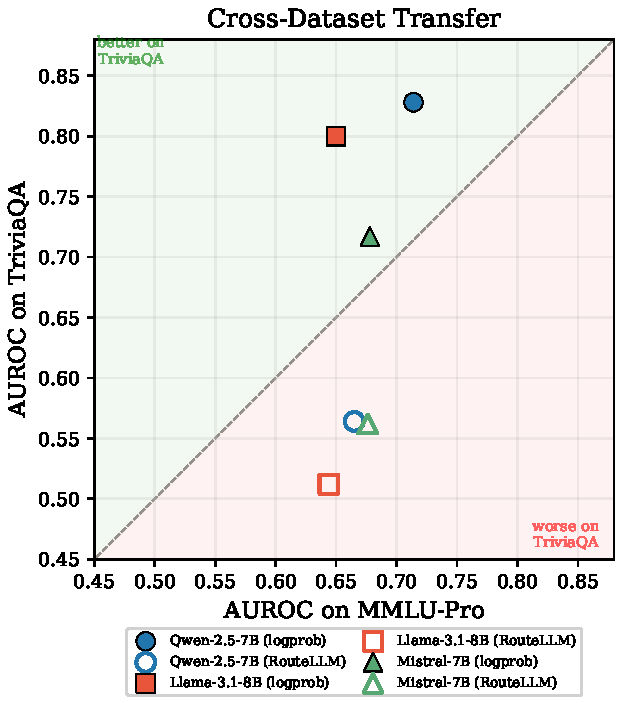
\includegraphics[width=0.85\columnwidth]{figures/fig1_cross_dataset.pdf}
\caption{Cross-dataset transfer. Filled markers: logprob (above diagonal = better on TriviaQA). Open markers: RouteLLM (below diagonal = collapses on TriviaQA).}
\label{fig:cross}
\end{figure}

\subsection{Supervised Learning Curve}
\label{sec:learning-curve}

\begin{table}[h]
\centering
\caption{RouteLLM-nm AUROC at increasing training sizes. Last row: logprob (zero-shot).}
\label{tab:lc}
\small
\begin{tabular}{rrrr}
\toprule
Training $N$ & Qwen & Llama & Mistral \\
\midrule
25 & 0.757 & 0.624 & 0.484 \\
50 & 0.511 & 0.470 & 0.624 \\
100 & 0.609 & 0.692 & 0.671 \\
250 & 0.654 & 0.681 & 0.566 \\
500 & 0.653 & 0.623 & 0.650 \\
${\sim}$1000 & 0.620 & 0.646 & 0.649 \\
\midrule
logprob (0) & \textbf{0.714} & \textbf{0.650} & \textbf{0.678} \\
\bottomrule
\end{tabular}
\end{table}

RouteLLM is unstable at small $N$ (swings of 0.15--0.20), converges around $N{=}250$--$500$, and at convergence never consistently exceeds the zero-shot line (\Cref{tab:lc}, \Cref{fig:lc}).

\begin{figure}[t]
\centering
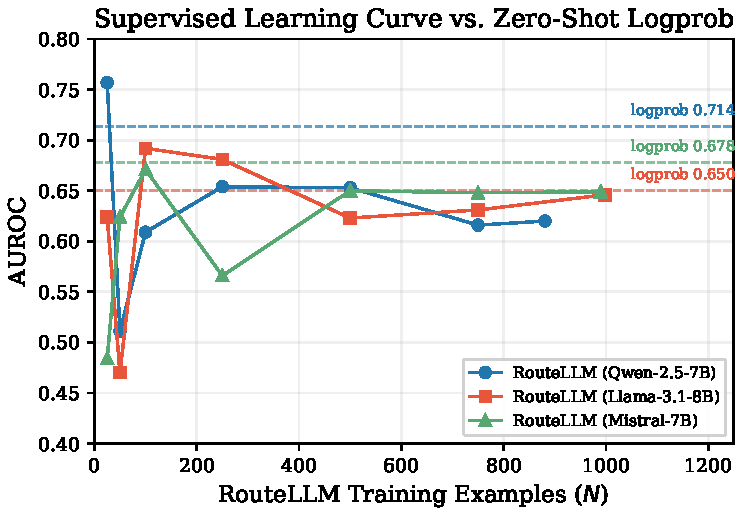
\includegraphics[width=0.95\columnwidth]{figures/fig2_learning_curve.pdf}
\caption{RouteLLM learning curve (solid) vs.\ logprob zero-shot AUROC (dashed), per model.}
\label{fig:lc}
\end{figure}

\subsection{Signal Latency}

\begin{table}[h]
\centering
\caption{Mean signal latency (ms). ``Pre-gen'' = routes before full local generation.}
\label{tab:latency}
\small
\begin{tabular}{lrrrc}
\toprule
Signal & Qwen & Llama & Mistral & Pre-gen? \\
\midrule
RouteLLM & $<$1 & $<$1 & $<$1 & \checkmark \\
KS (FAISS) & 72 & 72 & 77 & \checkmark \\
GSA v3 & 461 & 777 & 767 & \checkmark \\
logprob & 1{,}531 & 4{,}756 & 3{,}873 & $\times$ \\
SC & 539 & 2{,}874 & 2{,}766 & $\times$ \\
\bottomrule
\end{tabular}
\end{table}

Log-probability requires 1.5--4.8s of local generation before routing (\Cref{tab:latency}). A two-stage system can use GSA as a pre-generation filter (${\sim}$500ms) and logprob as a post-generation quality check.

\subsection{Naive Fusion Hurts}

\begin{table}[h]
\centering
\caption{AUROC of signal combinations (simple mean) vs.\ logprob alone.}
\label{tab:fusion}
\begin{tabular}{lrrr}
\toprule
Combination & Qwen & Llama & Mistral \\
\midrule
logprob alone & \textbf{0.714} & \textbf{0.650} & \textbf{0.678} \\
all 6 (mean) & 0.523 & 0.643 & 0.643 \\
logprob + GSA & 0.634 & 0.645 & 0.669 \\
\bottomrule
\end{tabular}
\end{table}

Mean fusion drags the strong signal toward weaker ones (\Cref{tab:fusion}). The effect is largest on Qwen where the quality gap is widest.

\subsection{Retrieval-Conditional Self-Assessment}
\label{sec:retrieval-gsa}

\begin{table}[h]
\centering
\caption{GSA v3 (retrieval-conditional) vs.\ v2 (bare) on Qwen MMLU-Pro ($n{=}931$).}
\label{tab:gsa}
\begin{tabular}{lrr}
\toprule
Variant & AUROC & Queries w/ retrieval \\
\midrule
GSA v2 (bare) & 0.562 & 0 / 931 \\
GSA v3 ($\tau{=}0.70$) & \textbf{0.599} & 290 / 931 (31\%) \\
GSA v3 ($\tau{=}0.60$) & 0.511 & 769 / 931 (83\%) \\
\bottomrule
\end{tabular}
\end{table}

Strong-hit-only retrieval ($\tau{=}0.70$) improves the signal by $+$0.037 (\Cref{tab:gsa}); including marginal hits ($\tau{=}0.60$) degrades it below the bare baseline. The design principle---never mention retrieval absence---is model-agnostic but density-dependent.

% ══════════════════════════════════════════════════════════════════
\section{Analysis}
\label{sec:analysis}

\subsection{Why Does Log-Probability Work?}
\label{sec:analysis-logprob}

Average token log-probability measures how surprised the model was by its own output. On factual QA, a model that ``knows'' the answer produces high-probability tokens; a model that is guessing produces lower-probability, higher-variance tokens \citep{kadavath2022language}.

\begin{table}[h]
\centering
\caption{Signal quality vs.\ RLHF emphasis.}
\label{tab:rlhf}
\begin{tabular}{llrr}
\toprule
Model & RLHF emphasis & logprob & GSA \\
\midrule
Qwen-2.5-7B & Calibration-aware & \textbf{0.714} & 0.562 \\
Mistral-7B & Mixed & 0.678 & 0.638 \\
Llama-3.1-8B & Helpfulness & 0.650 & \textbf{0.614} \\
\bottomrule
\end{tabular}
\end{table}

Models with calibration-aware RLHF produce stronger logprob signals (\Cref{tab:rlhf}). Models without benefit more from explicit self-assessment. The two signals are complementary across the model-family axis.

\subsection{Why Does Supervised Routing Collapse Cross-Dataset?}

RouteLLM learns which regions of embedding space correspond to easy queries on MMLU-Pro. This transfers across model families (Qwen-trained RouteLLM achieves 0.663--0.675 on Llama/Mistral) because query difficulty is partially model-agnostic. But the embedding structure of MMLU-Pro is specific to MMLU-Pro. TriviaQA occupies a different region with different difficulty patterns.

Log-probability measures a property of the model's generation, not of the query. It transfers because it does not depend on the query distribution.

\subsection{Why Does Fusion Hurt?}

Equal-weight fusion drags a strong signal toward weaker ones---a known failure mode when component quality is heterogeneous \citep{dietterich2000ensemble}. Thompson Sampling fusion, which should learn to upweight strong signals, collapses to equal-weight in our setup because no routing decisions are made during evaluation. Adaptive fusion with real feedback remains open.

\subsection{Knowledge Similarity: A Same-Dataset Confound}

KS is consistently inverted (AUROC 0.413--0.426). Per-category analysis reveals the mechanism: harder MMLU-Pro categories (law at 16.2\% accuracy, engineering at 29.2\%) have \emph{higher} retrieval similarity because the KB was seeded from the same distribution. A KB seeded from external sources would produce a different distribution. We did not test this.

% ══════════════════════════════════════════════════════════════════
\section{Cold-Start Deployment Guide}
\label{sec:deployment}

\begin{table}[h]
\centering
\caption{Routing options at deployment time.}
\label{tab:deploy}
\small
\begin{tabular}{llccc}
\toprule
Stage & Signal & AUROC range & Cost & Latency \\
\midrule
Day 0 & logprob & 0.650--0.833 & \$0 & 1.5--4.8s \\
Day 0 & GSA v3 & 0.562--0.720 & \$0 & 0.5--0.8s \\
After labeling & RouteLLM & 0.620--0.676 & ${\sim}$\$25 & $<$1ms \\
\bottomrule
\end{tabular}
\end{table}

\textbf{Recommendation.} Use logprob from the first query (\Cref{tab:deploy}). If latency is critical, add GSA as a pre-generation filter. RouteLLM training is only justified when (a)~the query distribution is known and stable, (b)~pre-generation routing is required, and (c)~cross-dataset transfer is not needed.

% ══════════════════════════════════════════════════════════════════
\section{Related Work}
\label{sec:related}

\textbf{Supervised routing.} RouteLLM \citep{ong2024routellm} trains classifiers on preference data. Extensions include contextual bandits \citep{chen2025adaptive}, bandit feedback \citep{soare2025bandit}, dueling feedback \citep{li2025dueling}, non-stationary pricing \citep{tabernermiller2026paretobandit}, and routing strategy surveys \citep{gomes2025routing}. All require training data. None benchmark against zero-shot alternatives.

\textbf{Uncertainty-based routing.} \citet{chuang2025confident} benchmark uncertainty-based SLM routing across 1{,}500+ settings. \citet{zhang2025uncertainty} propose confidence-driven edge-cloud routing. \citet{mukkunnoth2025confidence} combine three signals for pre-generation hallucination routing. Our work differs in directly comparing against supervised baselines and testing cross-dataset transfer.

\textbf{Activation probes for success prediction.} Most directly related to our work, \citet{lugoloobi2026encode} train linear probes on pre-generation hidden-state activations to predict whether a model will answer correctly, achieving AUROC ${>}0.7$ on math and coding tasks. They demonstrate probe-guided routing with up to 70\% cost reduction on MATH, and find that routing effectiveness is limited by probe reliability rather than routing sophistication---a conclusion we reach independently from a different direction. Critically, their approach requires access to model internals (residual-stream activations), limiting it to open-weight models with controlled inference. Our logprob signal requires only token probabilities available from any inference API, works zero-shot across model families without per-model probe training, and---as we show---transfers across datasets where supervised approaches fail. They do not compare against RouteLLM-style supervised baselines or test cross-dataset generalization.

\textbf{Token-level calibration.} \citet{kadavath2022language} showed calibrated token probabilities in RLHF'd models. \citet{guo2017calibration} established calibration theory. \citet{huang2024logprob} confirmed log-probability reliability in instruction-tuned models. We apply the same mechanism to routing and show it transfers where supervised approaches fail.

\textbf{Self-assessment.} \citet{kadavath2022language} tested P(True). \citet{ren2023selfeval} reformulated generation into self-evaluation. \citet{chen2024trust} found self-reported confidence outperforms self-consistency at lower cost. We extend self-assessment with retrieval-conditional prompting and show effectiveness is model-specific.

\textbf{Multi-signal uncertainty.} UQLM \citep{lin2025uqlm} and MUSE \citep{geng2025muse} combine signals into unified frameworks. We find naive fusion hurts---consistent with ensemble theory \citep{dietterich2000ensemble} under heterogeneous quality, but not previously shown for LLM routing.

\textbf{Self-consistency.} \citet{wang2022selfconsistency} proposed multi-path agreement. Our two-sample variant is model-specific: effective on Llama/Mistral, dead on Qwen.

\textbf{Semantic entropy.} \citet{kuhn2023semantic} proposed detecting confabulations via entropy over semantic clusters, published in \textit{Nature}. \citet{farquhar2024robust} extended this with cheaper approximations. These methods require 5--10 generations per query, making them 5--10$\times$ more expensive than our single-generation logprob signal.

\textbf{Verbalized confidence.} \citet{tian2023just} showed LLMs can express calibrated confidence when prompted. \citet{xiong2024llmsexpress} found verbalized confidence is often overconfident but improvable. Our GSA signal is a constrained variant that extracts YES-token probability rather than a numeric score, avoiding the overconfidence problem.

\textbf{Uncertainty surveys.} \citet{geng2024survey} and \citet{huang2025uncertainty} provide comprehensive surveys. Our work is narrower but deeper: fewer methods, more models and datasets, with a supervised baseline comparison that surveys do not include.

% ══════════════════════════════════════════════════════════════════
\section{Limitations}
\label{sec:limitations}

\begin{enumerate}[leftmargin=*,itemsep=2pt]
\item \textbf{Two datasets, one task type.} Both MMLU-Pro and TriviaQA are factual QA. Reasoning, creative, and multi-turn tasks are untested.
\item \textbf{Three models, one size.} All 7--8B. The calibration hypothesis predicts logprob improves with scale; untested.
\item \textbf{Post-generation routing cost.} Logprob requires full generation (1.5--4.8s) before routing. Wasted on escalated queries.
\item \textbf{Static KB.} All experiments use a frozen knowledge base. In production, the KB grows from escalations, making routing non-stationary.
\item \textbf{MCQ inflation.} MMLU-Pro's 10-option format gives a 10\% chance floor. TriviaQA partially addresses this.
\item \textbf{Label noise.} 13\% inter-judge disagreement. Absolute AUROC carries ${\sim}{\pm}0.05$ uncertainty; differential comparisons are robust.
\end{enumerate}

% ══════════════════════════════════════════════════════════════════
\section{Conclusion}
\label{sec:conclusion}

Training data is not necessary for effective LLM confidence estimation. Average token log-probability---a zero-shot signal available from the first query at zero cost---matches supervised baselines in-distribution and substantially outperforms them out-of-distribution. For practitioners deploying local-to-cloud routing: start with log-probability, skip the training, and invest engineering effort elsewhere.

% ══════════════════════════════════════════════════════════════════

\bibliography{references}

\end{document}
